% 2024-09-?? EFMI STC Timisoara, Romania conference paper presentation
% 10 minutes presentation.
% TODOs 
\iffalse
%- Ziele der Ontologie
- Studienunterklassen ausblenden
- ausführlichere Überschriften
- mehr text am anfang (Einleitung mit Gegenstand, Motivation, Zielstellung)
- running example: Konkreter Informationsbedarf
- Z.B. Welche Features haben typische Laborinformationssysteme
oder "In welchen Publikationen wurden CPOE-Systeme mit welchen Features evaluiert?"
Alternativ: "Gibt es Publikationen, in denen die Features von CPOE erläutert und ihr Nutzen evaluiert werden? Welche Features werden dort besprochen?"
- https://codemeta.github.io/
- https://citation-file-format.github.io/
- https://schema.org/SoftwareApplication
- mit Bildern
- medfloss.org ?
- highlighting auf unterschiedlichen Folien der Implementation oder Sprechblasen
\fi

%\documentclass[aspectratio=43]{beamer}
%\documentclass[aspectratio=169]{beamer}
\documentclass[aspectratio=1610,12pt]{beamer}

\usepackage[english]{babel}
\usepackage{booktabs} % fancy tables
\usepackage{tabulary} % tables with auto column length 
\usepackage{hyperref}
\usepackage{siunitx}

\usetheme{imise}
\author{\emph{Konrad Höffner}, Hannes Raphael Brunsch, Franziska Jahn,\\Prof. Alfred Winter}
%\title{The SNIK Ontology of Information Management in Hospitals}
\title{\large Visualising Paths for Exploratory Search\\in the Health IT Ontology}
\date{November 29, EFMI STC 2024, 11.15--11.25, Room K1}
\def\address{Härtelstraße 16-18, 04107 Leipzig, Raum 227}
\def\email{konrad.hoeffner@imise.uni-leipzig.de} 
\def\telephone{+49 341 97 16322}


\newcommand{\imageslide}[4][]
{
\newgeometry{margin=0cm,top=1em}
\begin{frame}[plain]{~~~~#2}
\vspace{0.2em}
\centering\includegraphics[width=0.995\textwidth,height=0.95\textheight,keepaspectratio]{#3}
\\#1
\note{#4}
\end{frame}
\restoregeometry
}

\newcommand{\imageslidebare}[1]
{
\newgeometry{margin=0cm,top=1em}
\begin{frame}[plain]
\centering\includegraphics[width=0.995\textwidth,height=0.995\textheight,keepaspectratio]{#1}
\end{frame}
\restoregeometry
}

\begin{document}

\begin{frame}
\titlepage
\end{frame}

%- https://codemeta.github.io/
%- https://citation-file-format.github.io/
%- https://schema.org/SoftwareApplication

\begin{frame}[plain]{HITO\footnote{Jahn F et al. 2023. \emph{A Linked Open Data–Based Terminology to Describe Libre/Free and Open-source Software: Incremental Development Study}. \url{http://dx.doi.org/10.2196/38861}}---Introduction}
\begin{itemize}
\item RDFS/OWL ontology
\item RDF knowledge graph
\item describe libre/free and open source software with Linked Open Data
\item goals: support health IT management, research and education
%\item application system types, e.g. \emph{Radiology Information System}
%\item software products, e.g. \emph{Bahmni}
%\item evaluation studies covering software products
\end{itemize}

\end{frame}

{
%\newgeometry{top=1em}
\begin{frame}[plain]{Metadata Attributes}
%\begin{itemize}
%\item usual metadata, such as license, 
%\end{itemize}
% L U R O
\centering\includegraphics[width=0.9\textwidth,height=0.9\textheight,trim={0cm 2cm 23.5cm 3cm}, clip, keepaspectratio]{img/2024-05-hito\_diagram.pdf}
\end{frame}
\restoregeometry
}

{
\newgeometry{margin=0.5cm,top=1em}
\begin{frame}{~~~~Health IT Specifics}
\begin{itemize}
\item application system types, e.g. \emph{Radiology Information System}, \emph{PACS}
\item supported enterprise functions, e.g. \emph{management of medical devices}
\item features, e.g. \emph{booking of examinations}
\item organizational units, user groups
\item evaluation studies including the software product
\end{itemize}
% L U R O
\centering\includegraphics[width=0.995\textwidth,height=0.995\textheight,trim={8.8cm 4.2cm 7.2cm 4.9cm}, clip, keepaspectratio]{img/2024-05-hito\_diagram.pdf}
\end{frame}
\restoregeometry
}

{
\newgeometry{margin=0cm,top=1em}
\begin{frame}[plain]{~~~~Catalogues, Classifieds and Citations}
\begin{itemize}
\item catalogue: a collection of classified entries, e.g. features extracted from \emph{WHO Classification of Digital Health Interventions v1.0}
\item classified: a summarizing term from a catalogue, e.g. \emph{manage orders}
\item citation: natural language description of a software product from the documentation, e.g. \emph{prescribe longhand}
\end{itemize}
% L U R O
\centering\includegraphics[width=0.995\textwidth,height=0.995\textheight,trim={9.5cm 9.4cm 5.99cm 0cm}, clip, keepaspectratio]{img/2024-05-hito\_diagram.pdf}
\end{frame}
\restoregeometry
}

%[trim={5cm 0 0 0},clip]
%\imageslide{The Health IT Ontology}{img/2024-05-hito\_diagram.pdf}{}{}
%\imageslide{The Health IT Ontology~~~~~~~~~~~~~~~~\url{https://hitontology.eu}}{img/2024-05-hito\_diagram.pdf}{}{}

%\begin{frame}[plain]{The Health IT Ontology (HITO)---Background}
%\begin{itemize}
%\only<1>{
%\item describe Libre/Free and Open Source software with Linked Open Data
%\item RDFS/OWL ontology
%\item RDF knowledge graph
%\item application systems and software products
%\item evaluation studies covering software products
%\item goals: support health IT management, research and education
%}
%\end{itemize}
%\hspace{-1.2em}\includegraphics[width=1.1\textwidth,height=0.95\textheight,keepaspectratio]{img/2024-05-hito\_diagram.pdf}
%\end{frame}

%\imageslide{Exploration Options: RDF Browser}{img/rickview-hito.png}{}{}
%\imageslidebare{img/cscmedchart-lodview.pdf}
{
\newgeometry{margin=0.2cm,top=1em}
\begin{frame}[plain]{~~~~Exploration with RDF Browser\footnote{https://github.com/KonradHoeffner/rickview}}
~\\
~\\
\begin{itemize}
\setlength\itemsep{1em}
%\item each resource (software product, feature, $\ldots$) has it's own URL
\item one resource and its direct neighborhood
\item traverse connections step by step
\item missing overview
\end{itemize}
\vspace{-9em}
\hspace{20em}
\centering\includegraphics[width=0.995\textwidth,height=\textheight,keepaspectratio]{img/cscmedchart-lodview.pdf}
\end{frame}
\restoregeometry
}


\imageslide{Faceted Search}{img/hitofaceted.png}{}{}

\begin{frame}{Complex Information Needs: Examples}
\emph{
\begin{itemize}
\item Which enterprise functions do typical Laboratory Information Systems support?
\item Which publications evaluate features of CPOE systems? Which features are covered?
\end{itemize}
}
\end{frame}

\imageslide{Vision}{img/idea.pdf}{}{}
%\imageslide{Implementation I}{img/hitogui.pdf}
%\imageslide{Implementation}{img/ast1.png}{}{}

\begin{frame}{Path to SPARQL Query}
\begin{table}[ht]
\centering
\begin{tabular}{@{}llll@{}}
\toprule
Type & Represented by & Example & Triple pattern \\ \midrule
vertex $w_i$ & HITO class & Study & $?x \ rdfs:subClassOf \ w_i$ \\
vertex $w_1$ & data type (first vertex, backwards) & First Author & $?x_2 \ rdfs:label \ x_1$ \\
vertex $w_n$ & data type (last, backwards) & First Author & $?x_{n-1} \ rdfs:label \ x_n$ \\
edge $p_i$ & property & first author & $?x_i \ p_i \ x_{i+1}$ \\
edge $p_i$ & property & first author & $?x_{i+1} \ p_i \ x_i$ \\ \bottomrule
\end{tabular}
\caption{RDF triple patterns as components of the final SPARQL query. Variables $?x_i$ denote the actual letter x and number $i$ (e.g. $?x_5$ ) while $p_i$ represents the URI of the property $p_i$, such as :firstAuthor.}
\end{table}
\end{frame}

%\imageslide{Results}{img/ast2.png}{}{}
%\imageslide{Filtering}{img/ast3.png}{}{}

%%\imageslide{Search \& Exploration: SNIK Graph}{img/snik-graph-full.png}{}{}

\iffalse
\newgeometry{margin=0cm,top=1em}
\begin{frame}[plain]{~~~~Domain}
% Information Management in Hospitals is a core topic for students of medical computer science.
% Unfortunately, there are many different views of the domain, whose relationship is often unclear, and the terminology is full of synonyms and homonyms.
% So this domain is difficult to learn for students. 
\end{frame}
\restoregeometry

%\imageslide{Synonyms}{img/wordcloud-synonym.png}{}{}

%\imageslide{Meta Model}{img/metamodel9s.pdf}{}{}

%\imageslide{Modelling Example}{img/bb-cio.pdf}{}{}

\newgeometry{margin=0cm,top=1em}
\begin{frame}[plain]{~~~~Transformation}
%\centering%\includegraphics[width=0.7\textwidth,keepaspectratio]{img/5star.png}
\end{frame}
\restoregeometry

%\newgeometry{margin=0cm,top=1em}
\begin{frame}[plain]{~~~~Storage/Query, Author, Interlink \& Browse}
\begin{columns}[t]
\column{.5\textwidth}
\centering
%\includegraphics[width=\textwidth]{img/virtuoso.png}
%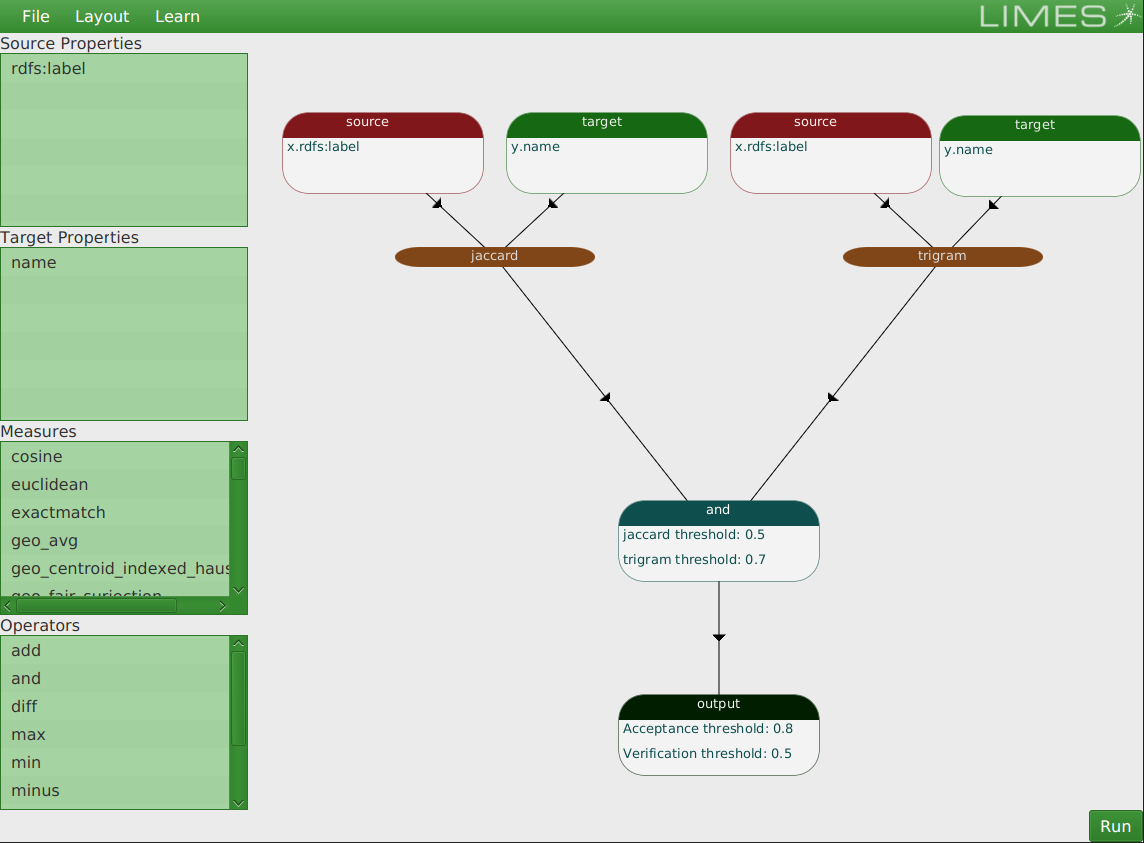
\includegraphics[width=\textwidth]{img/limes.png}
\column{.5\textwidth}
\centering
%\includegraphics[width=\textwidth]{img/ontowiki.png}
%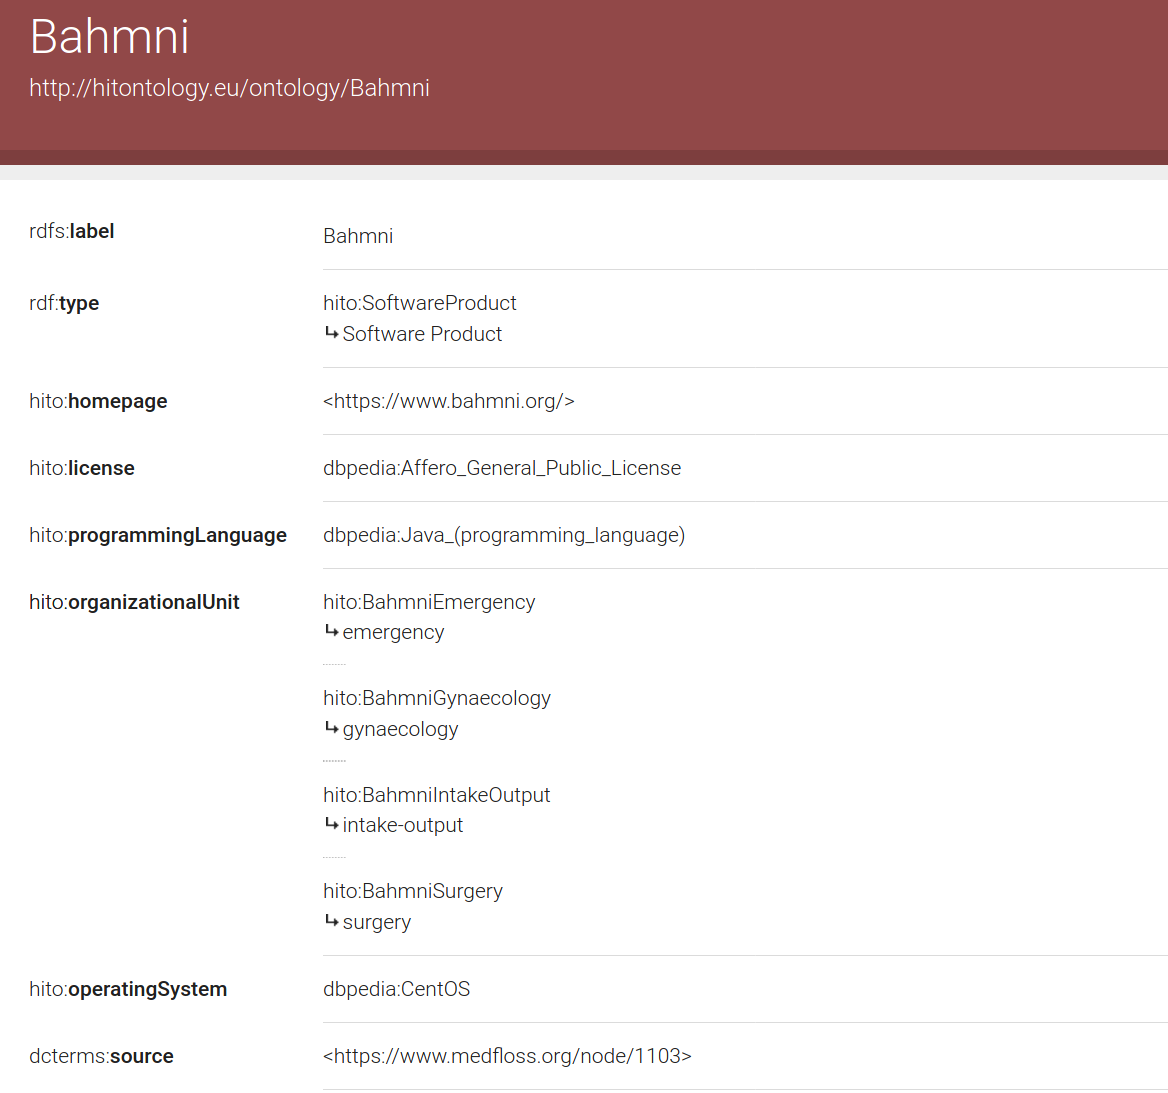
\includegraphics[width=\textwidth]{img/lodview.png}
\end{columns}
\end{frame}
\fi
%\restoregeometry

%\imageslide{Search \& Exploration: SNIK Graph}{img/snik-graph-full.png}{}{}

%\imageslide{Extraction}{img/5star.png}

\iffalse
\begin{frame}{Example Slide}
\begin{itemize}
\item 
\item 
\item 
\item 
\end{itemize}
\end{frame}

\begin{frame}[fragile]{Questions?}
\begin{itemize}
%\item Diese Präsentation \url{https://github.com/KonradHoeffner/latex/releases/download/colloquium/colloquium.pdf}
\vspace{0.5em}%here it works as intended
\item Visualization \url{https://hitontology.github.io/gui/}
\item GitHub \url{https://github.com/hitontology/gui}
\item HITO Project \url{https://hitontology.eu}
\item Contact \url{konrad.hoeffner@imise.uni-leipzig.de}
%\item SPARQL Endpunkt \url{http://www.snik.eu/sparql}
%\item RDF Browser \url{http://www.snik.eu/ontology}
%\item Evaluation \url{http://www.snik.eu/evaluation}
%\item Twitter \url{https://twitter.com/snik\_proj}
%\item Technisches Blog \url{https://imise.github.io/snik-ontology}
%\item GitHub Organisation mit Ticketsystem \url{https://github.com/imise}
\end{itemize}
\end{frame}

\fi
\end{document}
